\documentclass[
    a0paper,
    portrait,
    margin=3cm,
]{baposter}

\usepackage{wrapfig}
\usepackage{lmodern}
\usepackage{lipsum,graphicx}
\usepackage[T1]{fontenc}
\usepackage{amsmath}
\usepackage{amsthm}
\usepackage{amssymb}
\usepackage{enumitem}
\usepackage{xcolor}
\usepackage[algoruled,boxed,lined]{algorithm2e}
\newcommand{\theHalgorithm}{\arabic{algorithm}}
\usepackage{local-macros}
\usepackage{biblatex}
\renewcommand*{\bibfont}{\tiny}
\addbibresource{bibliography.bib}

\usepackage{wrapfig}

\selectcolormodel{RGB}

\graphicspath{{figures/}} % Directory in which figures are stored

\newtheorem{theorem}{Theorem}
\newcommand{\sol}{\textcolor{black}}
\newcommand{\solb}{\textcolor{black}}
\newcommand{\fel}{\textcolor{black}}
\newcommand{\HH}{\mathcal{H}}

\newcommand{\compresslist}{%
\setlength{\itemsep}{0pt}%
\setlength{\parskip}{1pt}%
\setlength{\parsep}{0pt}%
}

% ------------------------------------------------------------ 
% Theorem-like environments
% ------------------------------------------------------------ 
\newtheoremstyle{fancy} % name
        {0.7em}                    % Space above
        {0.5em}                    % Space below
        {\normalfont}                   % Body font
        {}                           % Indent amount
        {\bfseries\sffamily}                   % Theorem head font
        {}                          % Punctuation after theorem head
        {0.5em}                       % Space after theorem head
        {}  % Theorem head spec (can be left empty, meaning ‘normal’)
\newtheoremstyle{regular} % name
        {0.7em}                    % Space above
        {0.5em}                    % Space below
        {}                   % Body font
        {}                           % Indent amount
        {\bfseries\sffamily}                   % Theorem head font
        {}                          % Punctuation after theorem head
        {0.5em}                       % Space after theorem head
        {}  % Theorem head spec (can be left empty, meaning ‘normal’)
\swapnumbers

\theoremstyle{fancy} % default
% \newtheorem{name}[shared counter]{text}[upper counter]
\newtheorem{thm}{Theorem}
\newtheorem*{thm*}{Theorem}
\newtheorem{lemm}[thm]{Lemma}
\newtheorem*{lemm*}{Lemma}
\newtheorem{prop}[thm]{Proposition}
\newtheorem*{prop*}{Proposition}
\newtheorem{cor}[thm]{Corollary}
\newtheorem{corr}[thm]{Corollary}

\theoremstyle{regular}
\newtheorem{deff}[thm]{Definition}
\newtheorem{rem}[thm]{Remark}
\newtheorem{ex}[thm]{Example}
\newtheorem{axiom}[thm]{Axiom}
\newtheorem*{assump*}{Assumption}
\newtheorem{assump}[thm]{Assumption}

\newenvironment{boenumerate}
  {\begin{enumerate}\renewcommand\labelenumi{\textbf\theenumi.}}
  {\end{enumerate}}

% Make centered headers in the rectangle header style
\makeatletter
\renewcommand{\baposter@box@headerdrawtext@rectangle}[1]{
  \path (\baposter@box@name nw) +(0.5\boxwidth,-0.5\baposter@box@@boxheaderheight) node[anchor=center] {#1};%
}

\begin{document}

\definecolor{fgv_dark_blue}{RGB}{1, 62, 125}
\definecolor{fgv_light_blue}{RGB}{6, 143, 203}

\begin{poster}
{
    grid=false,
    headerborder=open, % Adds a border around the header of content boxes
    colspacing=.8em, % Column spacing
    bgColorOne=white, % Background color for the gradient on the left side of the poster
    bgColorTwo=white, % Background color for the gradient on the right side of the poster
    borderColor=fgv_light_blue, % Border color
    headerColorOne=fgv_dark_blue, % Background color for the header in the content boxes (left side)
    headerColorTwo=fgv_dark_blue, % Background color for the header in the content boxes (right side)
    headerFontColor=white, % Text color for the header text in the content boxes
    boxColorOne=white, % Background color of the content boxes
    textborder=rectangle, %rectangle, % Format of the border around content boxes, can be: none, bars, coils, triangles, rectangle, rounded, roundedsmall, roundedright or faded
    eyecatcher=false, % Set to false for ignoring the left logo in the title and move the title left
    headerheight=0.125\textheight, % Height of the header
    headershape=rectangle, % Specify the rounded corner in the content box headers, can be: rectangle, small-rounded, roundedright, roundedleft or rounded
    headershade=plain,
    headerfont=\Large\bf\sffamily\centering, % Large, bold and sans serif font in the headers of content boxes
    %textfont={\setlength{\parindent}{1.5em}}, % Uncomment for paragraph indentation
    linewidth=2pt, % Width of the border lines around content boxes
    columns=2,
}
{}
%
%----------------------------------------------------------------------------------------
%	TITLE AND AUTHOR NAME
%----------------------------------------------------------------------------------------
%
{
 %Sans Serif
{
    \vspace{1.3em}
    {\huge \sffamily Nonparametric Instrumental Variable Regression \\ through Stochastic Approximate  Gradient Descent}
    \vspace{.1em}
}
}
% {\vspace{0.2em} Add Author Name, Add another author name\\ 
% {\small \vspace{0.7em} Department of Computing, TU Dublin, Tallaght, 
{
        \small{Caio F. L. Peixoto$^1$, Yuri F. Saporito$^1$, Yuri R. Fonseca$^2$}
    {
        \vspace{0.1em} \\
        \small{$1.$ School of Applied Mathematics, FGV}
        \vspace{.1em} \\
        \small{$2.$ Columbia University}
        \vspace{.5em}
    }
}
{
    
\includegraphics[width=.27\linewidth]{emap_logo.png}
} % FGV emap logo


% this states the box starts at column 0 (edge of page), row 0 (top of page) for a span of 2 (columns wide)
\headerbox{1. Abstract}{name=abstract,column=0,row=0, span=1}{
    We propose SAGD-IV, an algorithm which performs \textbf{instrumental variable regression} through iterative \textbf{SGD-like updates in a\\ functional space}:
    \begin{itemize}[noitemsep]
        \item IV regression is formulated as a statistical inverse problem;
        \item A suitable risk functional is introduced;
        \item This risk is minimized directly using a first order procedure.
    \end{itemize}
    Convergence guarantees are obtained using \textbf{minimal assumptions} when compared to other NPIV models.
}

\headerbox{2. NPIV problem formulation}{name=npiv,column=0,below=abstract,span=1}{
    \vspace{-1em}
    \begin{equation}
        \label{iv equation}
        Y = \hstar ( X ) + \varepsilon, \quad \mean [ \varepsilon \mid X ] \neq 0, \quad X\notindep Z \quad \text{and} \quad \mean [ \varepsilon \mid Z ] = 0
        \vspace{-.5em}
    .\end{equation}
    For example, consider the market of interstate transportation.
    Take
    \begin{center}
        \begin{tabular}{cc}
            $ X = $ Bus ticket price & $ Y = $ Bus ticket sales \\
            $ Z = $ Gas price & $ \varepsilon =  $ Other market forces
        \end{tabular}
    \end{center}
    % \begin{equation*}
    %     X = \text{Bus ticket price} \quad Y = \text{Bus ticket sales}
    %     \quad Z = \text{Gas price} \quad \varepsilon = \text{Other market forces}
    % .\end{equation*}

    Let $ L^2 ( X ) = \left\{ h : \mean [ h ( X )^2 ] < \infty \right\} $.
    Then (\ref{iv equation}) is equivalent to
    \begin{equation}
        \label{operator equation}
        r = \meanop [ \hstar ]
    ,\end{equation}
    where $ r ( Z ) = \mean [ Y \mid Z ] $ and $ \meanop : L^2 ( X ) \to L^2 ( Z ) $ is given by
    \begin{equation*}
        \meanop [ h ] ( Z ) = \mean [ h ( X ) \mid Z ]
    .\end{equation*}
    Equation (\ref{operator equation}) motivates us to define the risk
    \begin{equation*}
        \risk ( h ) \defeq \mean [ \loss ( r ( Z ), \meanop [ h ] ( Z ) ) ]
    .\end{equation*}
    We compute the gradient explicitly:
    \begin{equation*}
       \nabla \risk ( h ) ( x )
       = \meanop^{ * } [ \partial_{ 2 } \loss ( r ( \cdot ), \meanop [ h ] ( \cdot ) ) ] ( x )
       = \mean [ \Phi ( x, Z ) \partial_{ 2 } \loss ( r ( Z ), \meanop [ h ] ( Z ) ) ]
    ,\end{equation*}
    where $ \Phi ( x, z ) = \frac{ p_{ XZ } ( x, z ) }{ p_{ X } ( x ) p_{ Z } ( z ) } $.
    % Hence,
    % \begin{equation*}
    %     \nabla \risk ( h ) \approx \Phi ( \cdot , Z ) \partial_{ 2 } \loss ( r ( Z ), \meanop [ h ] ( Z ) ) 
    % .\end{equation*}
    We estimate $ \Phi, r $ and $ \meanop $ with $ \hat{ \Phi }, \hat{ r } $ and $ \hat{ \meanop } $ and look for a solution in a convex, closed and bounded set $ \searchset \subseteq L^2 ( X ) $.
}

\headerbox{3. Algorithm}{name=algorithm, column=1}{
    % After computing the gradient descent update, we apply $ \pi_{ \searchset } $, an orthogonal projection onto $ \searchset $.

    % The final average is taken due to good theoretical properties.

    \begin{algorithm}[H]\label{algo: sagdiv}
        \caption{SAGD--IV}
        \SetKwInOut{Input}{input}
        \SetKwInOut{Output}{output}
        \Input{
            Samples $ \left\{ ( \bz_{ m } )_{ m=1 }^{ M } \right\} $.
            Estimators $ \hat{ \Phi }, \hat{ r } $ and $ \hat{ \meanop } $.
            Sequence of learning rates $ ( \alpha_{ m } )_{ m=1 }^{ M } $.
        }
        \Output{ $ \hat{ h } $ }
        \For{$ 1 \leq m \leq M $}{
        Set $ u_{ m } = \hat{ \Phi } ( \cdot , \bz_{ m } ) \partial_{ 2 } \ell \left( \hat{ r } ( \bz_{ m } ), \hat{ \meanop } [ \hat{ h }_{ m - 1 } ] ( \bz_{ m } ) \right) $ \;
        Set $ \hat{ h }_{ m }  = \pi_{ \searchset } \left[
            \hat{ h }_{ m-1 } - \alpha_{ m } u_{ m }  
        \right] $ \;
    }
    Set $ \hat{ h } = \frac{ 1 }{ M } \sum_{ m=1 }^{ M } \hat{ h }_{ m } $ \;
    \end{algorithm}
}

\headerbox{4. Convergence Rate}{name=theorem,column=1, span=1, below=algorithm}{
    \vspace{6pt}
    \begin{align*}
        \alpha &= \norm{ \Phi - \hat{ \Phi } }_{ L^{ 2 } ( \prob_{ X } \otimes \prob_{ Z } ) }^2 + \norm{ r - \hat{ r } }_{ L^2 ( Z ) }^2 + \norm{ \meanop - \hat{ \meanop } }_{ \op }^2, \\
        \xi &= \frac{ 3 }{ 2 } \norm{ \hat{ \Phi } }_{ \infty }^2 \left(
            C_{ 0 }^2 + L^2 \norm{ \hat{ r } }_{ L^2 ( Z ) }^2 + L^2 D ^2 \norm{ \hat{ \meanop } }_{ \op }^2
        \right), \\
        \tau &= 2 D \max \left\{
            3 ( C_{ 0 }^2 + L^2 \mean [ Y^2 ] + L^2 D^2 ),
            2L^2 \norm{ \hat{ \Phi } }_{ \infty }^2,
            2L^2 D^2 \norm{ \hat{ \Phi } }_{ \infty }^2
        \right\}
    .\end{align*}
    Then, under suitable assumptions on $ \loss, \searchset, \meanop $ and the estimators $ \hat{ \Phi }, \hat{ r }, \hat{ \meanop } $, we have
    \begin{align*}
        \mean_{ \bz_{ 1:M } } \left[
            \risk ( \hat{ h } ) - \risk ( \hstar )
        \right]
        \leq \frac{ D^2 }{ 2 M \alpha_{ M } }
        + \frac{ \xi }{ M } \sum_{ m=1 }^{ M } \alpha_{ m }
        + \tau \sqrt{ \alpha }.
    \end{align*}
    \vspace{7pt}

    This suggests that the learning rate should satisfy the usual conditions:
    \begin{equation*}
        M \alpha_{ M } \to \infty \quad \text{and} \quad \frac{ 1 }{ M } \sum_{ m=1 }^{ M } \alpha_{ m } \to 0
    .\end{equation*}
}

\headerbox{5. Numerical Experiment}{name=experiment,column=0,span=2,below=npiv}{

    {
        We compare our method with Kernel Instrumental Variable Regression (KIV) \cite{singh2019}.
        \begin{center}
            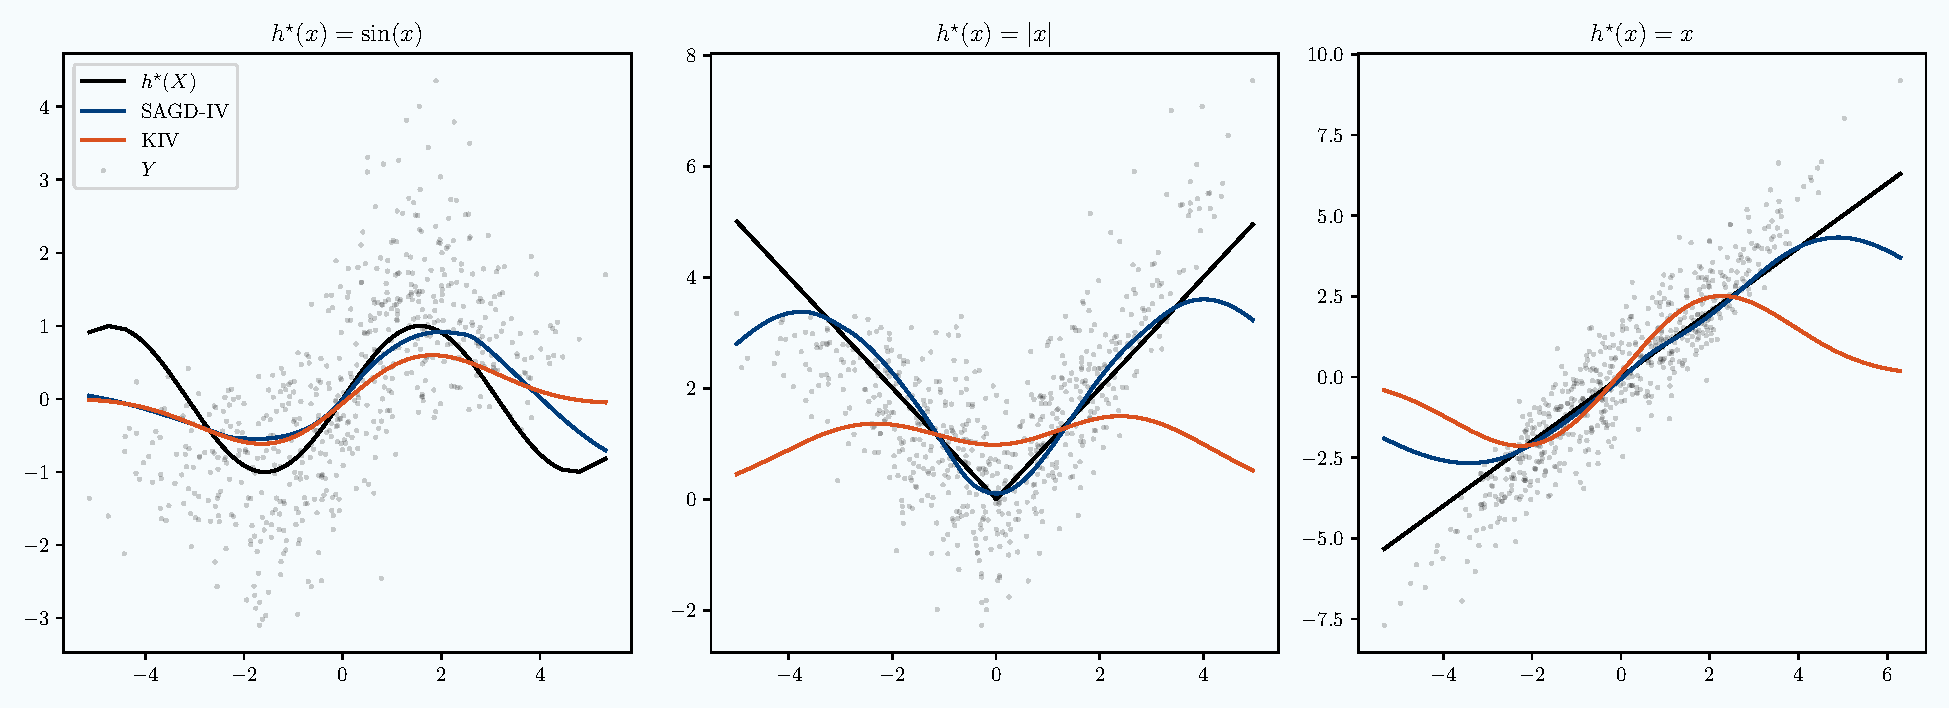
\includegraphics[width=\textwidth]{sagdiv_kiv_comparison.pdf}
        \end{center}
    }

}

\headerbox{6. Next Steps}{name=next-steps,column=0,below=experiment, above=bottom,span=1}
{
    \vspace{1em}
    \begin{itemize}[noitemsep]
        \item More thorough benchmarks;
        \item Application to discrete outcomes: $ Y = \ind \left\{ \hstar ( X ) + \varepsilon > 0 \right\} $;
        % \item Explore more options for $ \hat{ \Phi }, \hat{ r } $ and $ \hat{ \meanop } $.
    \end{itemize}
}

\headerbox{7. References}{name=references,column=1,below=experiment,above=bottom,span=1}{
    \nocite{sagd, yuri2022}
    \printbibliography[heading=none]
}

\end{poster}

\end{document}
